\documentclass[12pt]{article}
\usepackage{fullpage}
\usepackage{float}
\usepackage{graphicx}
\usepackage{subcaption}
\usepackage{amsmath}
\usepackage{algpseudocode}
\usepackage{algorithm}


\begin{document}
\title{Notes on Domain Decomposition}
\author{Scott Aiton}
\maketitle

\section{Forming Schur Complement Matrix}

If there is a $\gamma$ for each point on the interface, how to we determine the values?

\begin{figure}[H]
    \centering
    \includegraphics[width=2in]{abgamma2.pdf}
    \caption{figure with l and r}
\end{figure}

We want the flux going out of ouf the $l$ cell to match the flux going into the $r$ cell.
So we get the equation:
\begin{equation}
\gamma-l=r-\gamma
\end{equation}
or:
\begin{equation}
2\gamma-(l+r)=0
\end{equation}
Note that $l$ and $r$ are not constants, but are dependent on the value of $\gamma$.
So, let's change them to the be functions of $\gamma$:
\begin{equation}
2\gamma-(L(\gamma)+R(\gamma))=0
\end{equation}
So now we have a function of $\gamma$:
\begin{equation}
F(\gamma)=2\gamma-(L(\gamma)+R(\gamma))
    \label{function}
\end{equation}
Therefore we have a function that we want to find the zero of this function:
\begin{equation}
F(\gamma)=0
\end{equation}

If we have a single $\gamma$ value that we are solving for, this function becomes a linear equation of the form:
\begin{equation}
F(\gamma)=a\gamma-b
\end{equation}
we can find the coefficients by:
\begin{align}
    b&=-F(0)\\
    a&=F(1)+b
\end{align}
With these coefficients, we can solve for $\gamma$
\begin{align}
F(\gamma)=0\\
a\gamma-b=0\\
a\gamma=b\\
\gamma=\frac{b}{a}
\end{align}
When there are multiple interface points, then we have a system of linear equations:
\begin{equation}
F(\gamma)=A\gamma-b
\end{equation}
the $b$ vector is found by
\begin{equation}
b=-F(0)
    \label{bvec}
\end{equation}
each column of the matrix is found by
\begin{equation}
A(:,i) = F(e_i)+b
    \label{matrixcol}
\end{equation}
we can then determine the  $\gamma$ vector by solving
\begin{equation}
A\gamma=b
\end{equation}

\section{Quick Formation of the Schur Complement Matrix}
In this section, we can use the process described in equation \eqref{matrixcol} to derive an algorithm
that allow us to quickly form the Schur compliment matrix.
\paragraph{The matrix does not depent on the RHS}
First, let's reconsider equations  \eqref{bvec} and \eqref{matrixcol}. If we are solving on a system
where the rhs and lhs on each patch is zero, the $b$ vector for the Schur complement matrix will
be $0$, since $0$ is the correct solution for the interfaces. So equation \ref{matrixcol} turns into
\begin{equation}
    A(:,i) = F_{zero}(e_i)
\end{equation}
where $F_{zero}$ is the same as equation \ref{function} but with the rhs on each domain replaced 
with $0$.
So now we use can use this to reduce the amount of work needed to form the Schur complement matrix.
\\
\\
Let's consider what happens when we solve for $F_{zero}(e_i)$. If a single interface value is set
to $1$, only the two adjacent domains will have non-zero dirichlet boundary conditions, meaning that
only the two adjacent domains will have non-zero solutions. This means that when we are solving for 
$F_{zero}(e_i)$, we can  assume that solution on any domain that is not adjacent to the interface
with the $1$ is zero. In other words, we only have to do a solve on the two adjacent domains, rather
than solving for all the domains.

\paragraph{Indexing of $\gamma$ Values} 
If the individual values in the $\gamma$ vector are indexed in the following way:
\begin{itemize}
    \item If the interface is on the east or west side of the patch, the $\gamma$ values will be indexed consecutively from the bottom up.
    \item If the interface is on the north or south side of the patch, the $\gamma$ values will be indexed consecutively from left to right.
\end{itemize}
Since the $\gamma$ values on each interface indexed consecutively, the Schur complement matrix takes
on a block structure, where each block is $n\times n$.
\paragraph{Sparsity}

Consider the example grid given in Figure \ref{2domain}.
When a single $1$ is set on the interface $i_{\textnormal{main}}$, only 7 interfaces will end up
having non-zero values: the main interface, $i_{\textnormal{main}}$, and the 6 auxiliary
interfaces, 
$i_{\textnormal{left north}}$, $i_{\textnormal{left south}}$, $i_{\textnormal{left west}}$,
$i_{\textnormal{right north}}$, $i_{\textnormal{right east}}$, and $i_{\textnormal{right south}}$.

\begin{figure}[H]
    \centering
    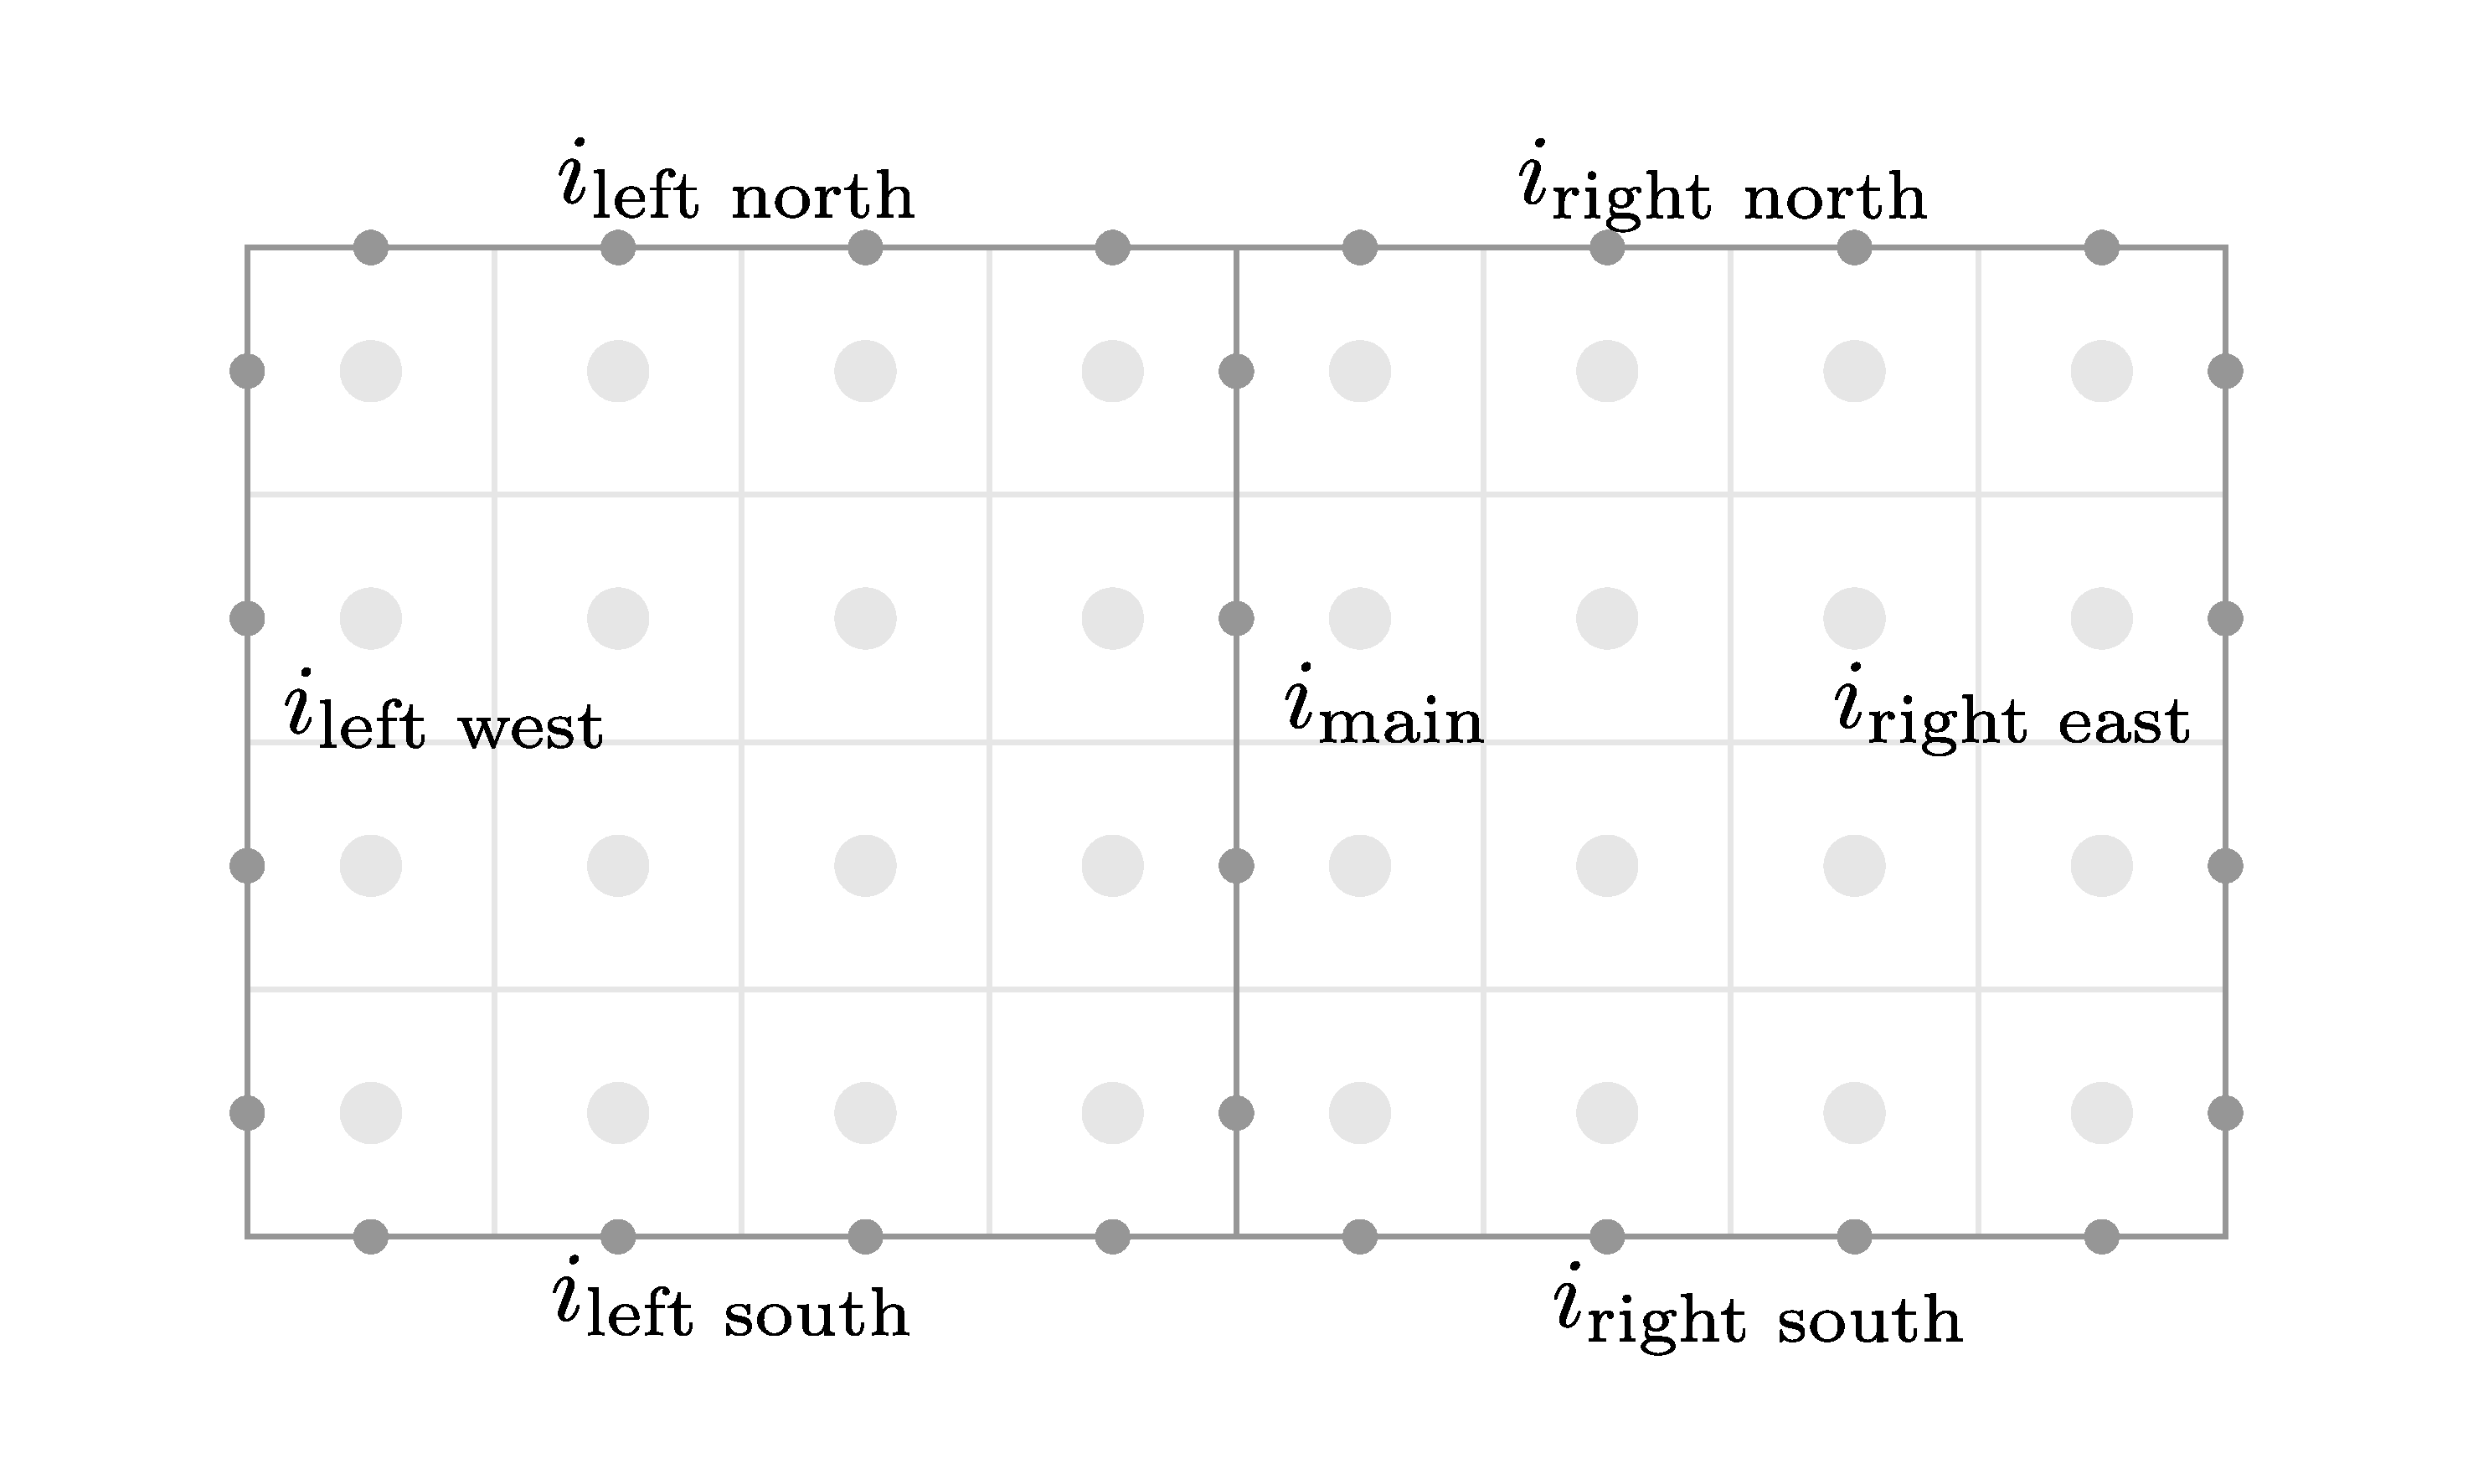
\includegraphics[width=6in]{images/2domain.pdf}
    \caption{Two domain example}
    \label{2domain}
\end{figure}

\paragraph{Splitting up the work}

If we look at equation \ref{function}, we can split up the work and process the two domains at
different times.
\begin{align}
    F_{left}(\gamma)&=\gamma-L(\gamma) \label{function_left}\\
    F_{right}(\gamma)&=\gamma-R(\gamma) \label{function_right}
\end{align}

So, when we process the left and right domains, we use equations \ref{function_left} and 
\ref{function_right}, respectively, for the diagonal blocks ($i_{\textnormal{main}}$).
When we are forming the matrix, we will insert the diagonal
block twice, summing the coefficients of one block into the other.

\paragraph{Rotation}
\begin{figure}[H]
    \centering
    \begin{subfigure}[b]{0.30\textwidth}
        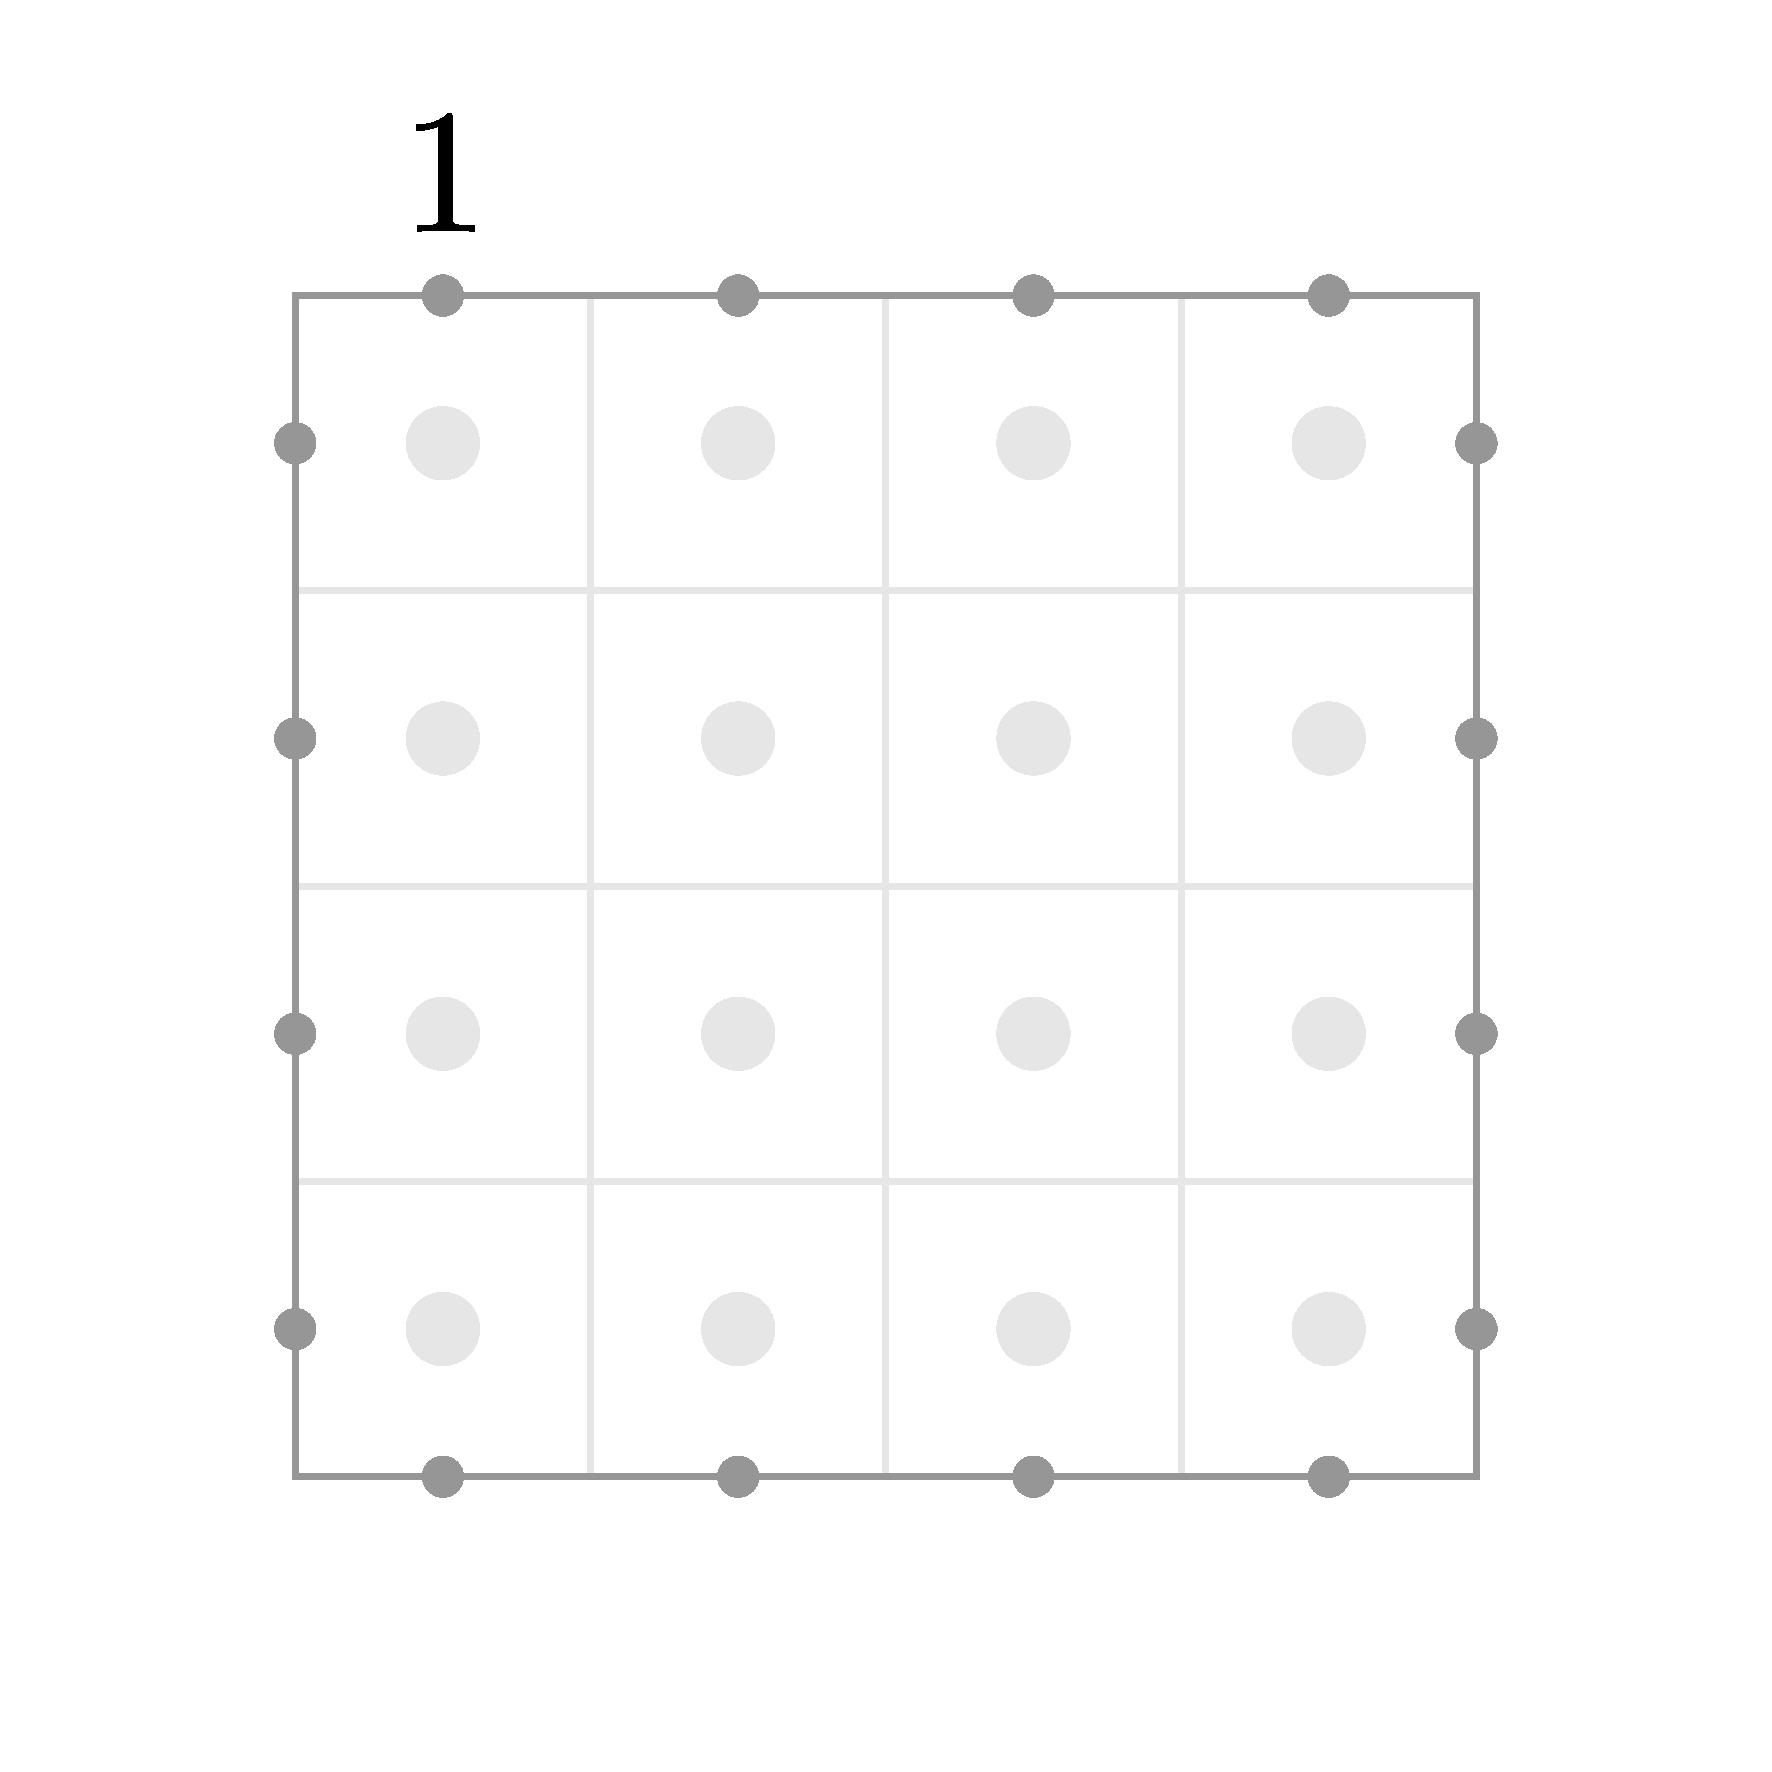
\includegraphics[width=\textwidth]{images/north1.pdf}
        \caption{North}
    \end{subfigure}
    \begin{subfigure}[b]{0.30\textwidth}
        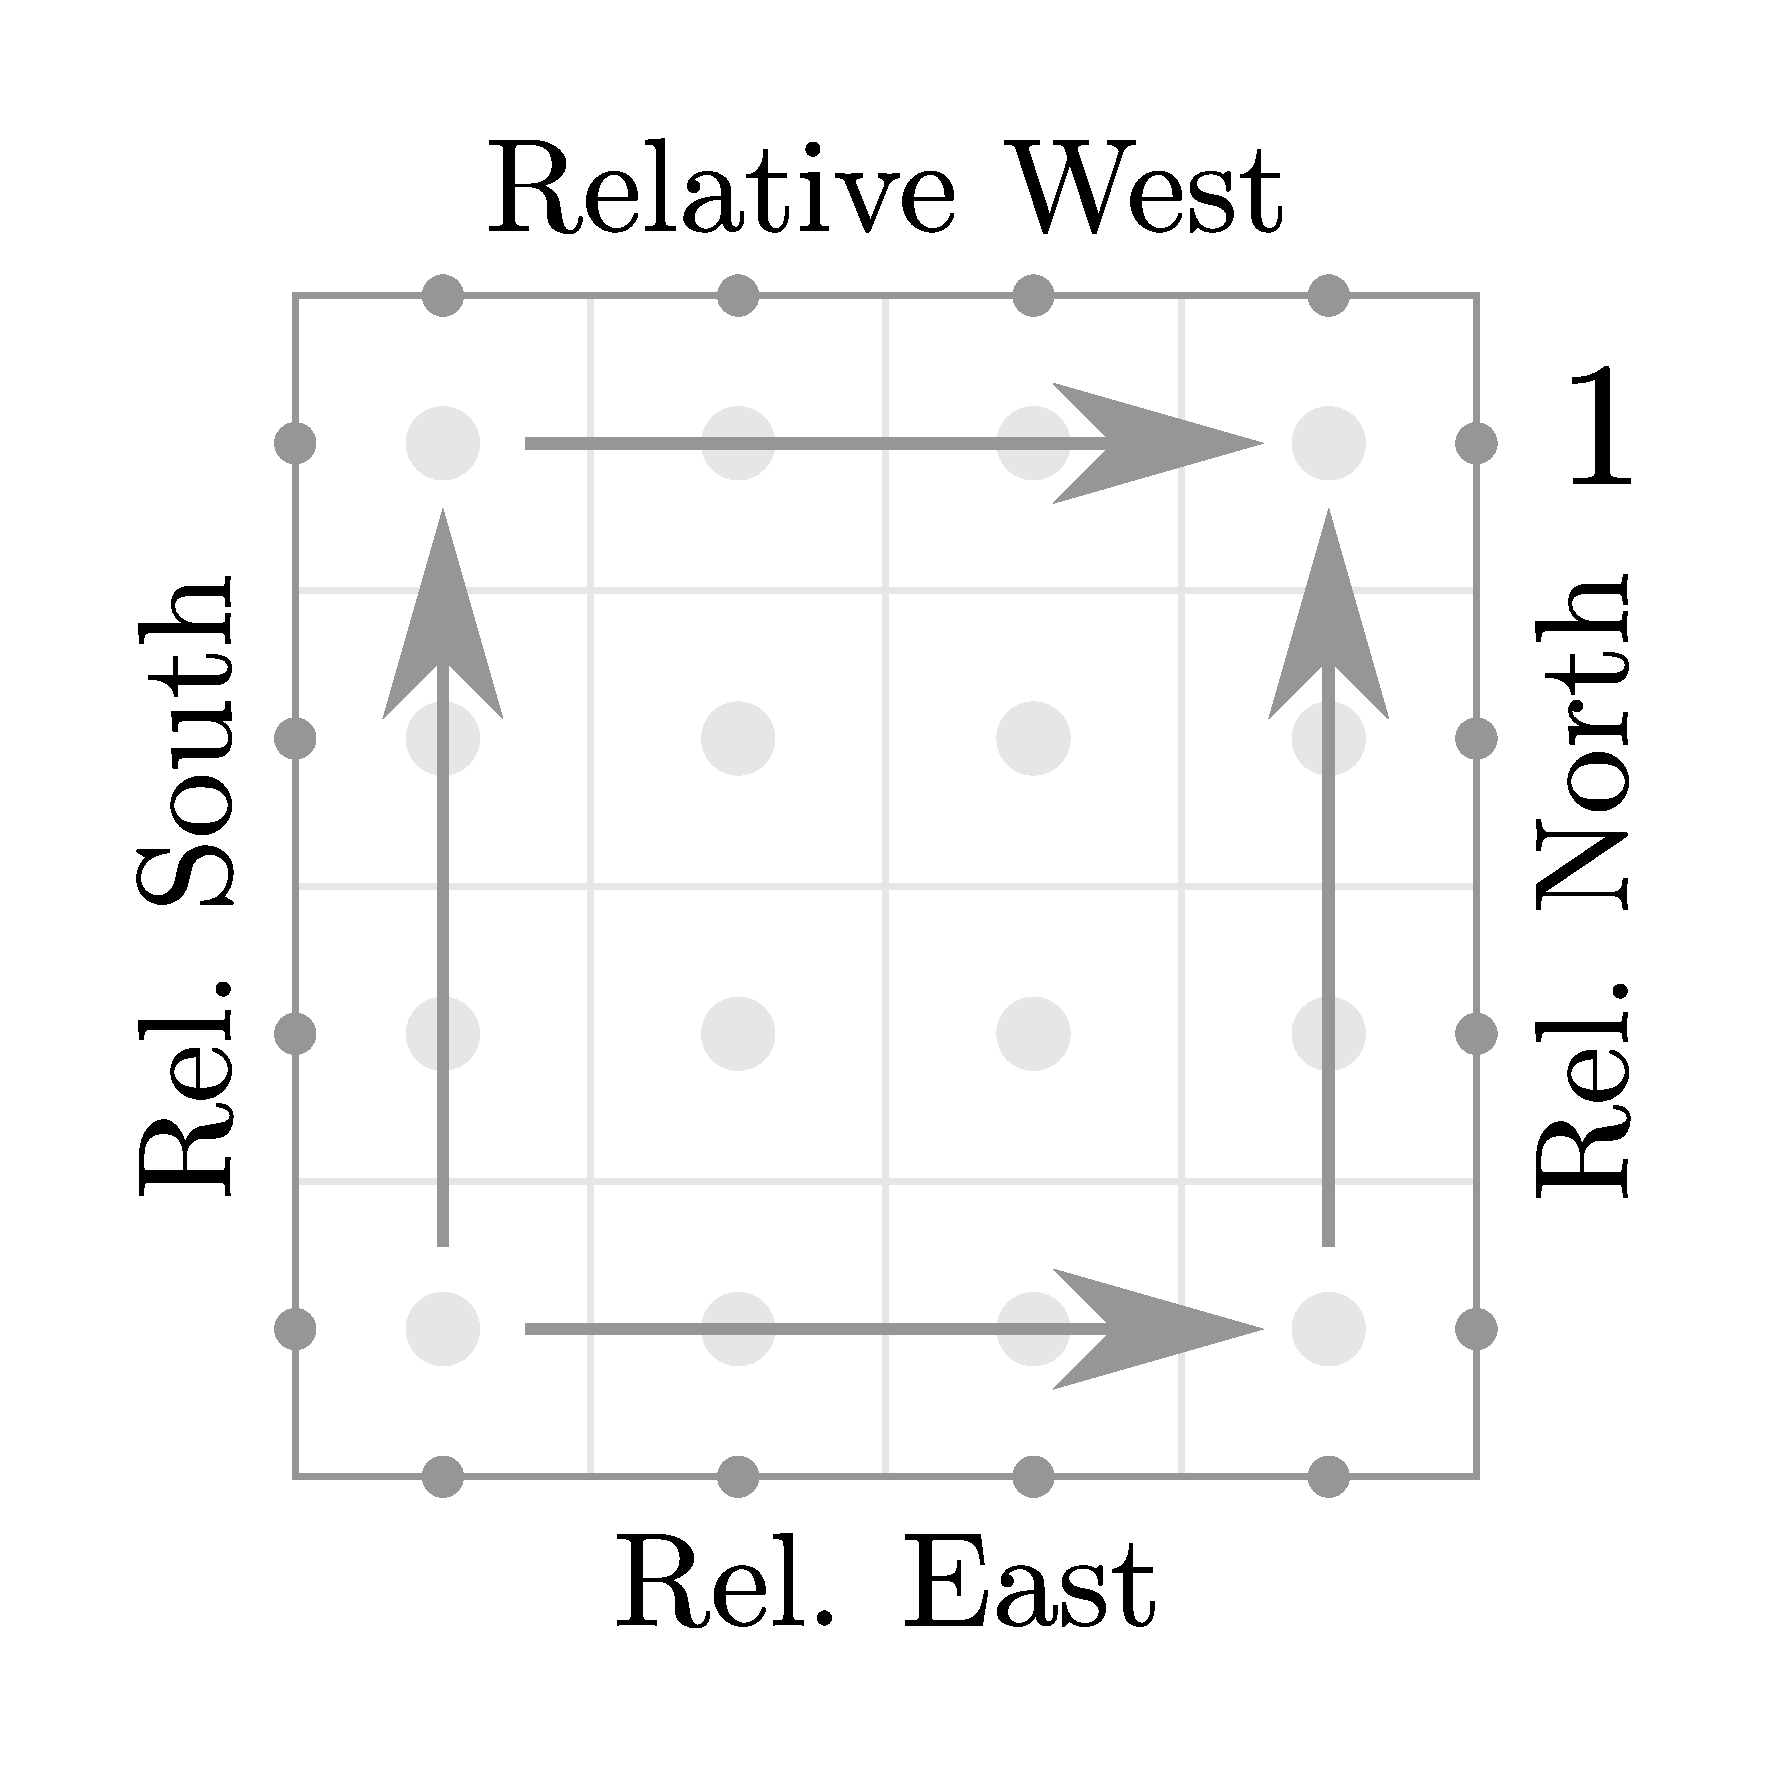
\includegraphics[width=\textwidth]{images/east1.pdf}
        \caption{East}
    \end{subfigure}
    \begin{subfigure}[b]{0.30\textwidth}
        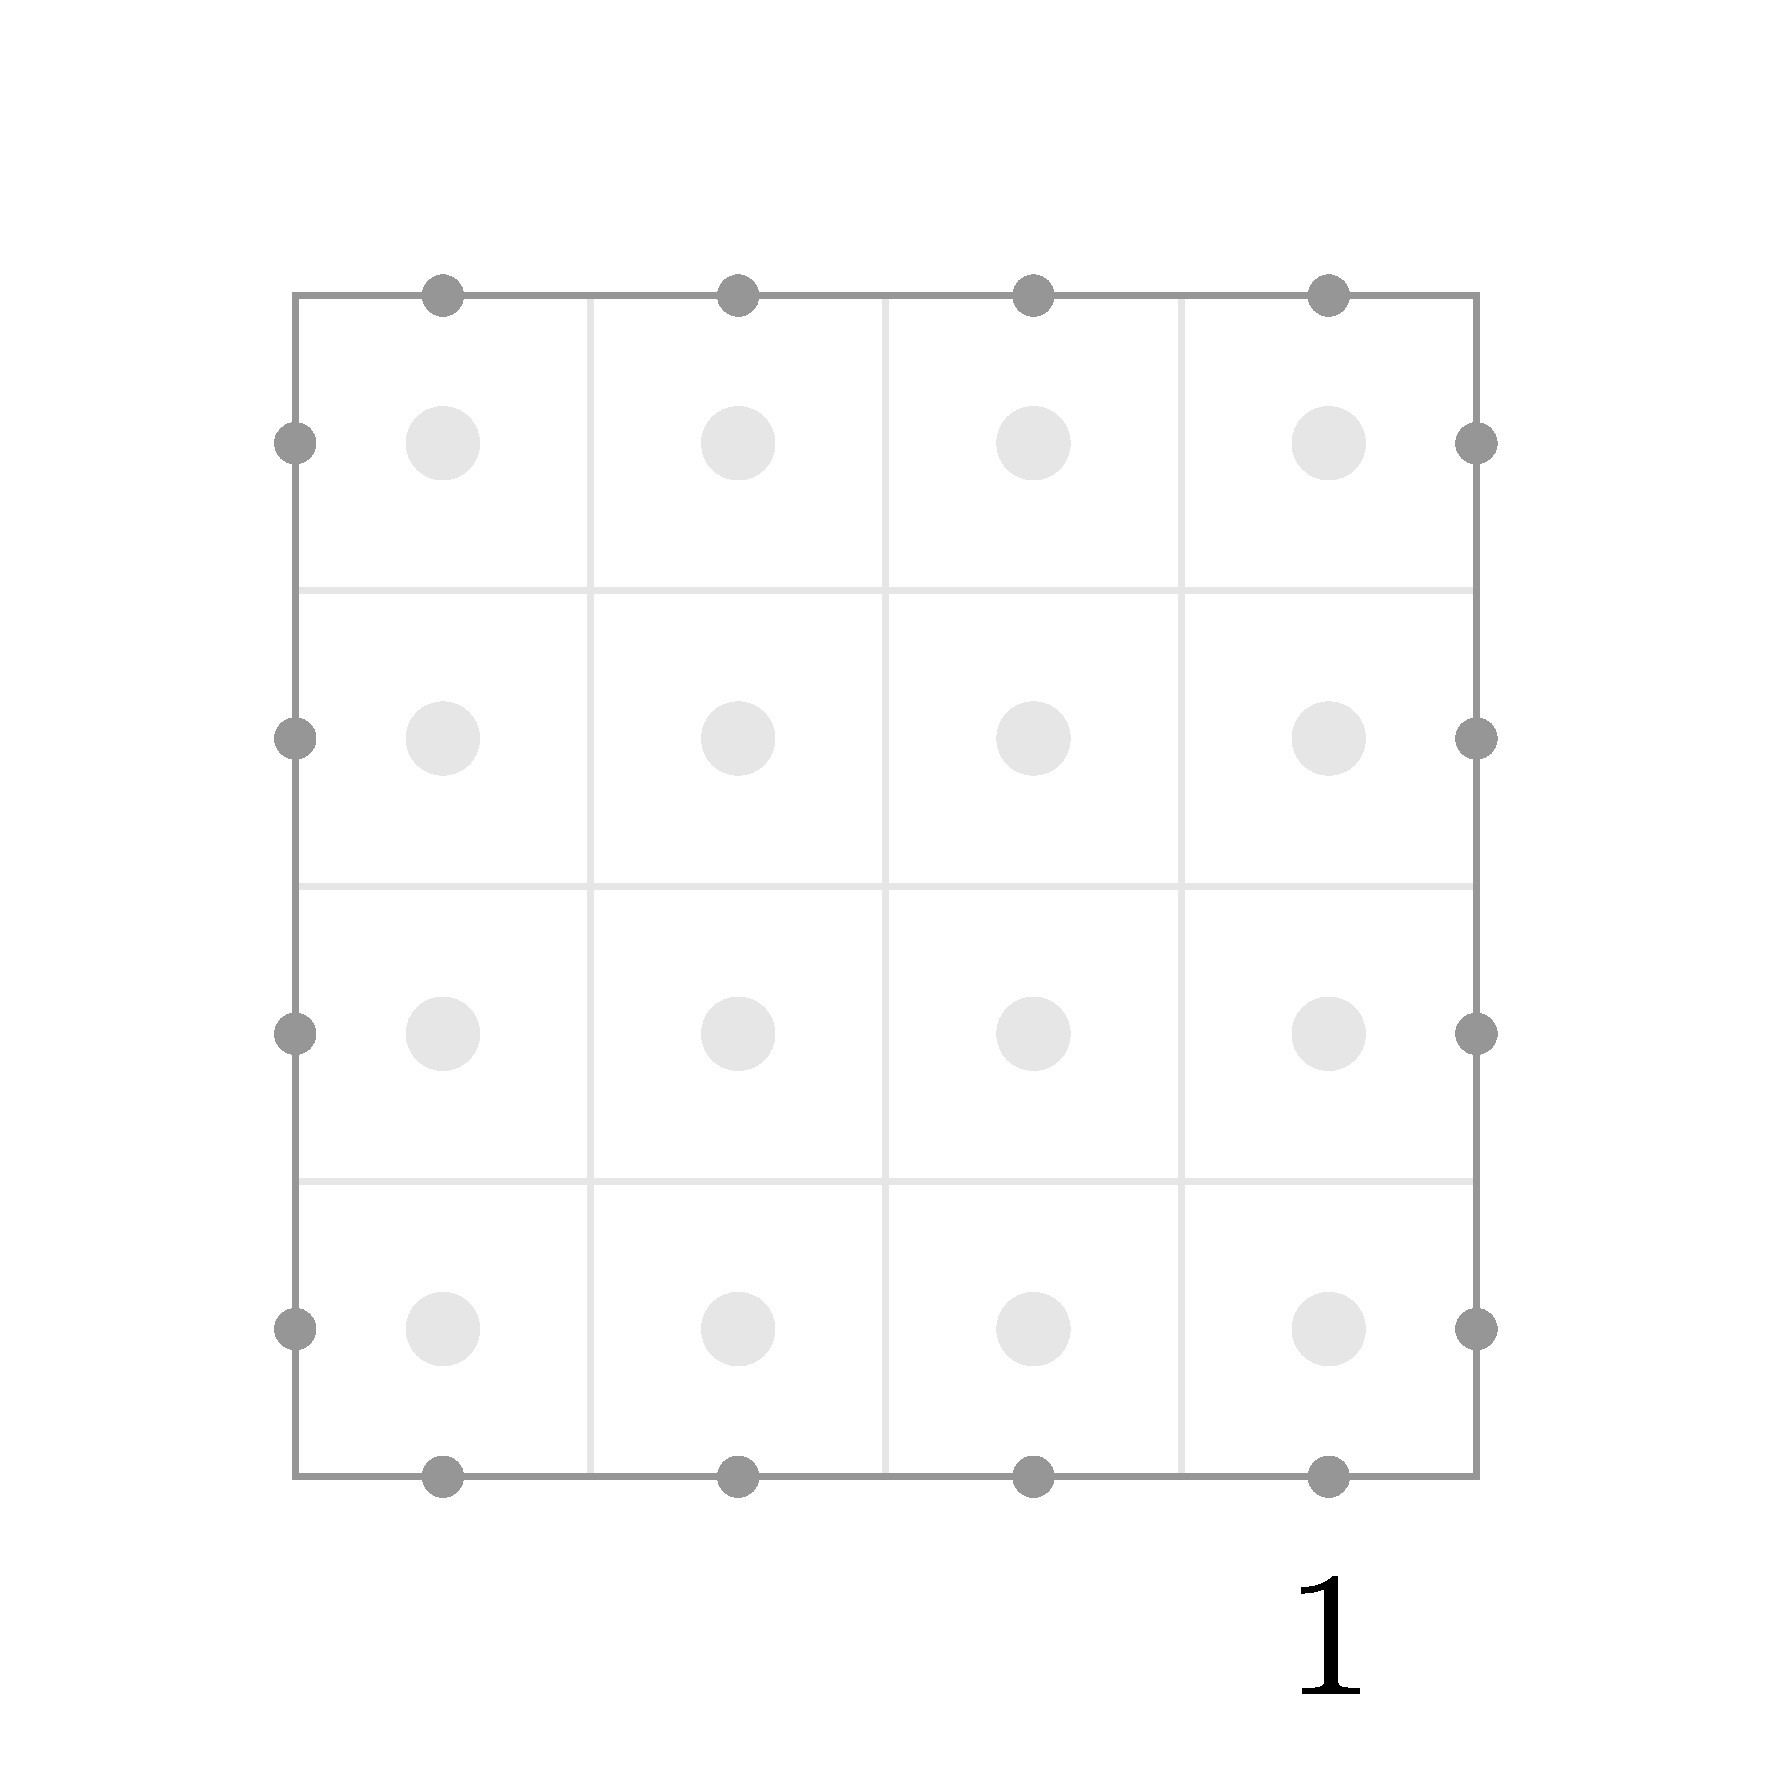
\includegraphics[width=\textwidth]{images/south1.pdf}
        \caption{South}
    \end{subfigure}
    \begin{subfigure}[b]{0.30\textwidth}
        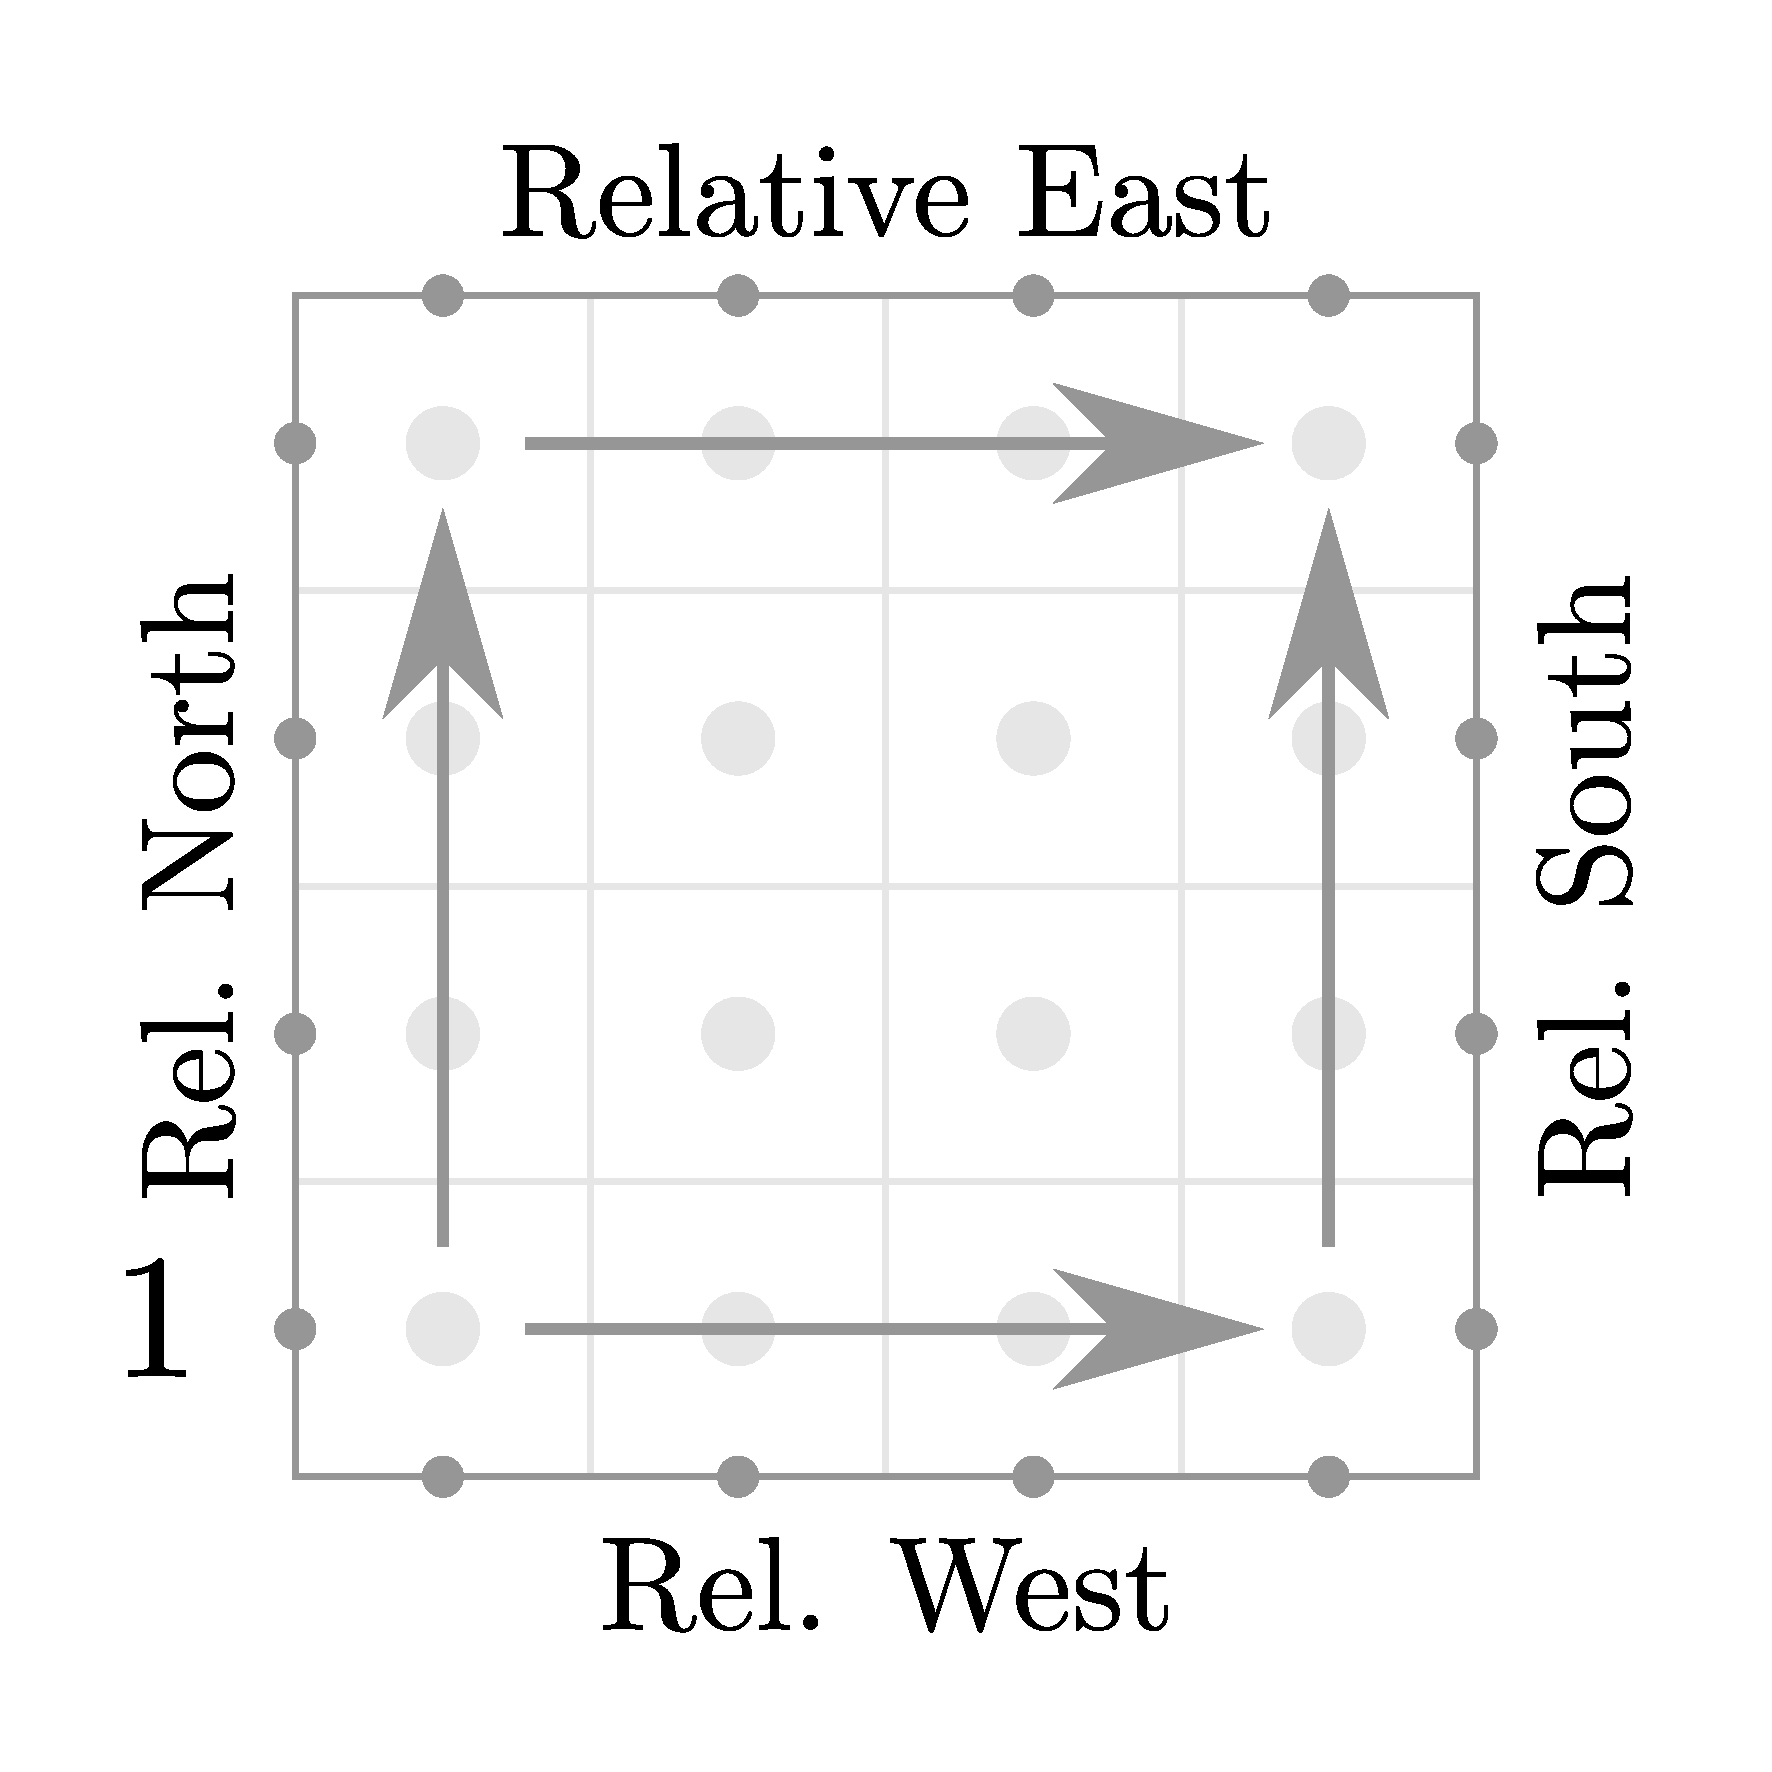
\includegraphics[width=\textwidth]{images/west1.pdf}
        \caption{West}
    \end{subfigure}

    \caption{Rotation}
    \label{rotation}
\end{figure}

Let the north side be our canonical side. Lets consider part a in figure \ref{rotation} where the
first $\gamma$ value on the north interface is set to $1$. If rotate this domain clockwise by $90$
degrees, that is equivalent to setting the last $\gamma$ value on the east interface to $1$. If we
rotate it again, it is equivalent to setting the last $\gamma$ value on the south interface to
$1$. And if we rotate once more, it would be equivalent to setting the first $\gamma$ value on the
east interface. 

This means that when we can get to coefficients for the blocks in the Schur complement matrix, by
setting each $\gamma$ value along the north interface to $1$, and then reuse these coefficients for
the interfaces on the other sides.



\paragraph{Algorithm}

%\begin{algorithm}
%\caption{Quick Schur Compliment Formation}
\begin{algorithmic}[1]
    \Procedure{FormMatrix}{Domains}
    \State $tbp \gets \emptyset$ \Comment{Set of interfaces to be processed}
    \ForAll{$\Omega \in Domains$}
        \If{$\Omega.northIndex \not= null$}
            \State $iface()$ \Comment{New iface object}
            \State $iface.side \gets North$
            \State $iface.northIndex \gets \Omega.northIndex$
            \State $iface.eastIndex \gets \Omega.eastIndex$
            \State $iface.southIndex \gets \Omega.southIndex$
            \State $iface.westIndex \gets \Omega.westIndex$
            \State $tbp.insert(iface)$
        \EndIf
        \If{$\Omega.eastIndex \not= null$}
            \State $iface()$ \Comment{New iface object}
            \State $iface.side \gets East$
            \State $iface.northIndex \gets \Omega.eastIndex$
            \State $iface.eastIndex \gets \Omega.southIndex$
            \State $iface.southIndex \gets \Omega.westIndex$
            \State $iface.westIndex \gets \Omega.northIndex$
            \State $tbp.insert(iface)$
        \EndIf
        \If{$\Omega.southIndex \not= null$}
            \State $iface()$ \Comment{New iface object}
            \State $iface.side \gets South$
            \State $iface.northIndex \gets \Omega.southIndex$
            \State $iface.eastIndex \gets \Omega.westIndex$
            \State $iface.southIndex \gets \Omega.northIndex$
            \State $iface.westIndex \gets \Omega.eastIndex$
            \State $tbp.insert(iface)$
        \EndIf
        \If{$\Omega.westIndex \not= null$}
            \State $iface()$ \Comment{New iface object}
            \State $iface.side \gets West$
            \State $iface.northIndex \gets \Omega.westIndex$
            \State $iface.eastIndex \gets \Omega.northIndex$
            \State $iface.southIndex \gets \Omega.eastIndex$
            \State $iface.westIndex \gets \Omega.southIndex$
            \State $tbp.insert(iface)$
        \EndIf
    \EndFor
    \State $\Omega()$
    \State $\Omega.rhs \gets 0$
    \State $\Omega.northBoundary \gets 0$
    \State $\Omega.eastBoundary \gets 0$
    \State $\Omega.southBoundary \gets 0$
    \State $\Omega.westBoundary \gets 0$
    \State $NorthBlock(n*n)$ \Comment{Allocate blocks of size n*n}
    \State $EastBlock(n*n)$
    \State $SouthBlock(n*n)$
    \State $WestBlock(n*n)$
    \For{$i \gets 1,n$}
         \State $\Omega.northBoundary(i) \gets 1$
         \State $\Omega.solve()$
         \State $NorthBlock(:,i) \gets \Omega.northBoundary-\Omega.lhs(:,n)$
         \State $EastBlock(:,i) \gets -\Omega.lhs(n,:)$
         \State $SouthBlock(:,i) \gets -\Omega.lhs(:,1)$
         \State $WestBlock(:,i) \gets -\Omega.lhs(1,:)$
    \EndFor
    \State $A()$ \Comment{Allocate Matrix}
    \ForAll{$iface \in tbp$} \Comment{Insert Blocks into Matrix}
        \State $reverseColumns \gets False$
        \State $reverseRows \gets False$
        \If {iface.side = East \textbf{or} iface.side = South}
             \State $reverseColumns \gets True$
        \EndIf
        \State
        \State $j \gets iface.northIndex$
        \State $A.insertBlock(NorthBlock,j,j,reverseColumns,reverseRows)$
        \State
        \If{$\Omega.southIndex \not= null$}
            \State $i \gets iface.southIndex$
            \State $A.insertBlock(SouthBlock,i,j,reverseColumns,reverseRows)$
        \EndIf
        \State
        \If {iface.side = South \textbf{or} iface.side = West}
             \State $reverseRows \gets True$
        \EndIf
        \State
        \If{$\Omega.eastIndex \not= null$}
            \State $i \gets iface.eastIndex$
            \State $A.insertBlock(EastBlock,i,j,reverseColumns,reverseRows)$
        \EndIf
        \State
        \If{$\Omega.westIndex \not= null$}
            \State $i \gets iface.westIndex$
            \State $A.insertBlock(WestBlock,i,j,reverseColumns,reverseRows)$
        \EndIf
        \State
    \EndFor
    \EndProcedure
\end{algorithmic}
%\end{algorithm}




\section{Handling Refinement}
We want the flux going out of the coarse cell to match the fluxes going into 
the fine cells.

\begin{figure}[H]
    \centering
    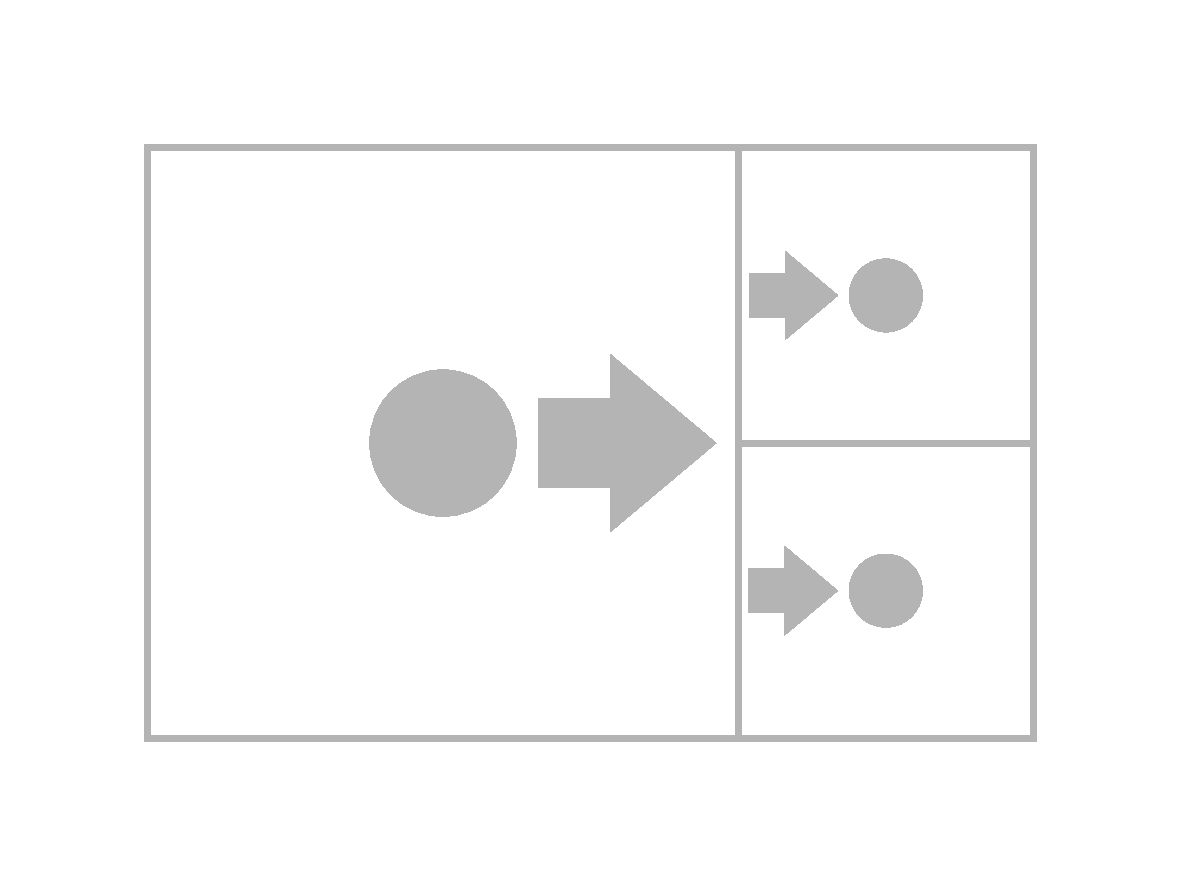
\includegraphics[width=4in]{images/amrflux.pdf}
    \caption{flux}
\end{figure}

We can represent this with the equation:

\begin{equation}
    \Phi_{c}=\Phi_{f_1}+\Phi_{f_2}
    \label{fluxconsv}
\end{equation}

\subsubsection*{Coming up with a stencil}
Lets say we want to find the ghost values for the coarse cell, the first fine cell, and the second
fine cell. Labeled $g_c$,$g_{f_1}$,and $g_{f_2}$, respectively.

\begin{figure}[H]
    \centering
    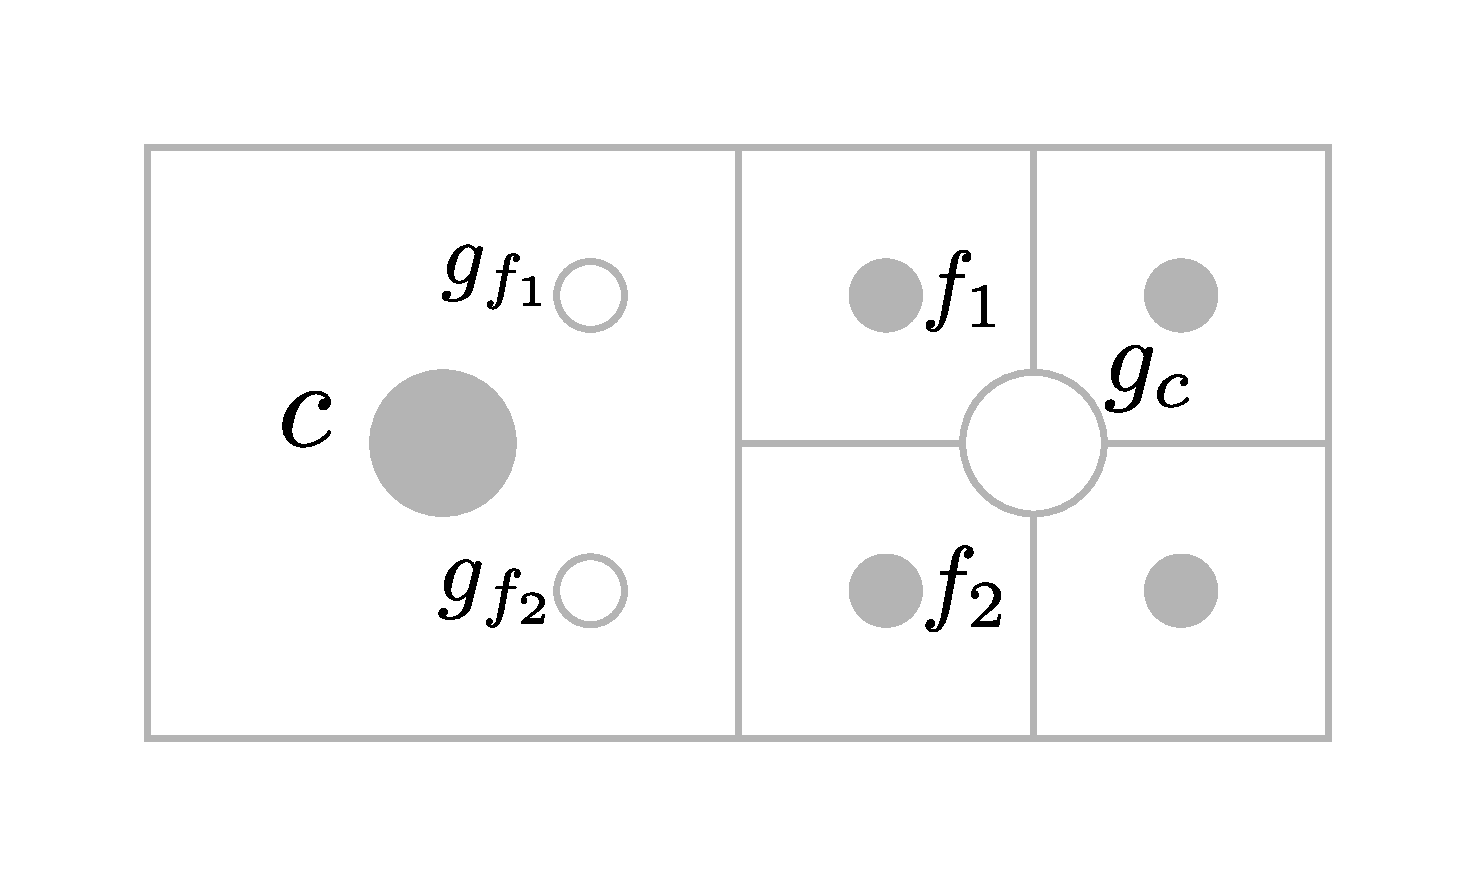
\includegraphics[width=4in]{images/ghost.pdf}
    \caption{ghost points}
\end{figure}

We can enforce flux conservation by interpolating to the fine ghost points, and then using equation
\ref{fluxconsv} to find the ghost point for the coarse cell.

The fluxes for each cell will be:
\begin{align}
    \Phi_c&=g_c-c\\
    \Phi_{f_1}&=f_1-g_{f_1}\\
    \Phi_{f_2}&=f_2-g_{f_2}
\end{align}

We can then solve for the value of $g_c$:

\begin{align}
    \Phi_{c}&=\Phi_{f_1}+\Phi_{f_2}\\
    g_c-c   &=f_1-g_{f_1}+f_2-g_{f_2}\\
    g_c     &=c+f_1-g_{f_1}+f_2-g_{f_2}
    \label{ghostconsv}
\end{align}

\subsubsection*{Bilinear interpolation}

Bilinear interpolation for the fine ghost points works, but error is not continuous.

TODO: Explain this and show an example

\subsubsection*{Quadratic interpolation}



\begin{figure}[H]
    \centering
    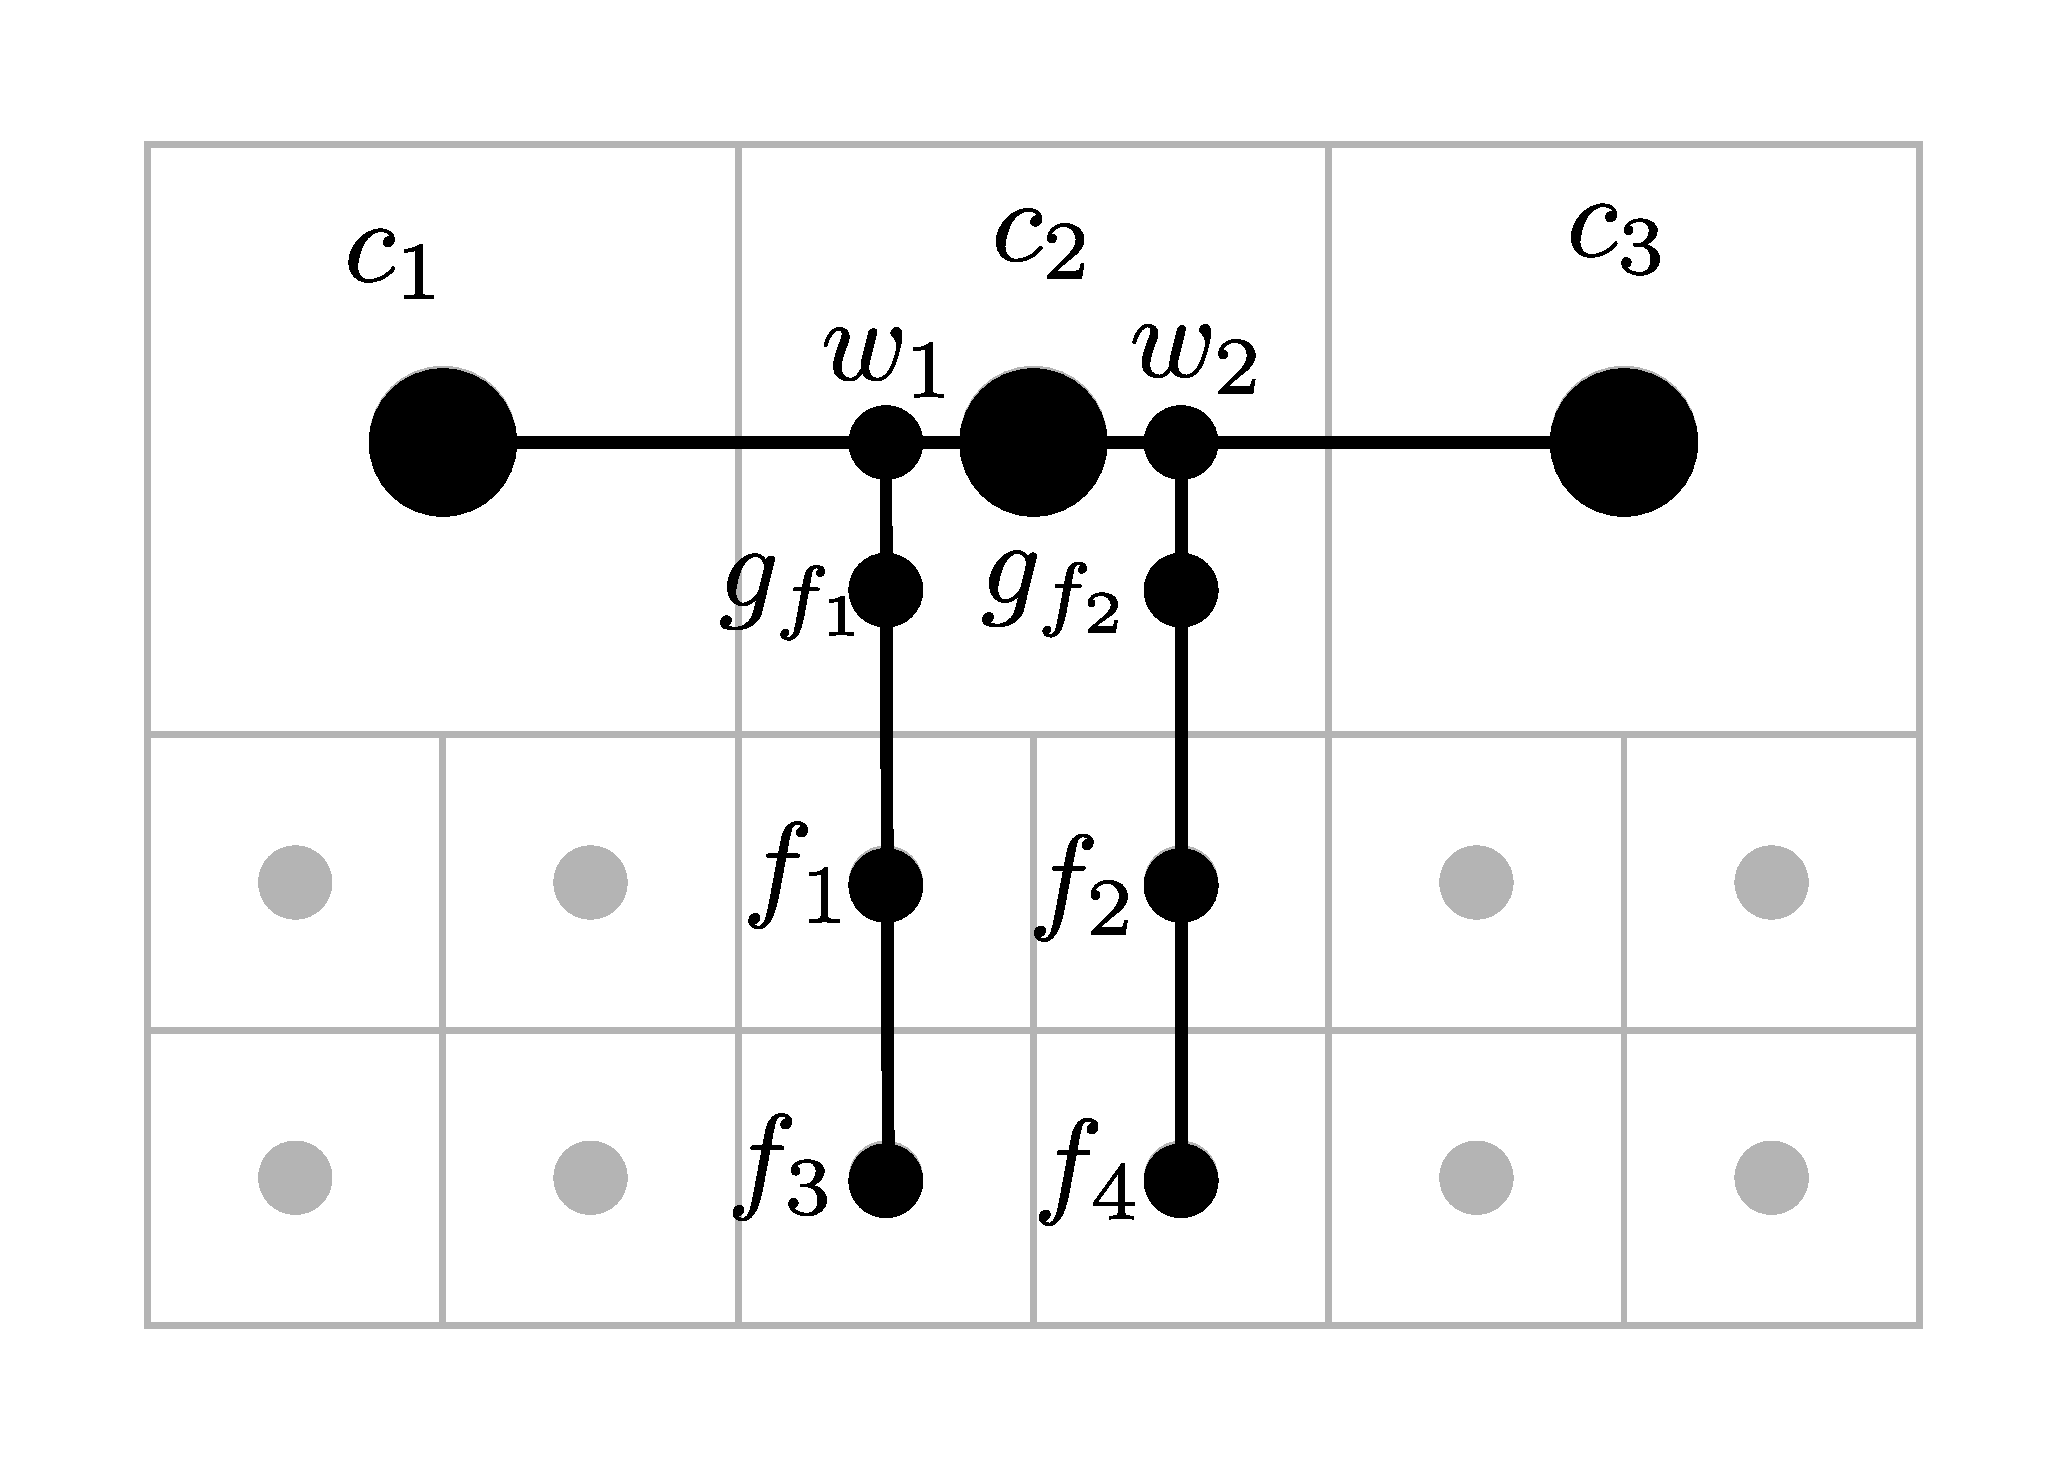
\includegraphics[width=5in]{images/quadstencil.pdf}
    \caption{flux}
\end{figure}

To find the value of $g_{f_1}$, we first use quadratic interpolation with the points 
$c_1$, $c_2$, and $c_3$ to interpolate to $w_1$:
\begin{equation*}
    w_1=\frac{5}{32}c_1+\frac{15}{16}c_2-\frac{3}{32}c_3
\end{equation*}
We then use quadratic interpolation with the points 
$w_1$, $f_1$, and $f_3$ to interpolate to $g_{f_1}$:
\begin{equation*}
    g_{f_1}=\frac{8}{15}w_1+\frac{2}{3}f_1-\frac{1}{5}f_3
\end{equation*}
Plug in the value for $w_2$, and we get the final equation for $g_{f_1}$:
\begin{equation*}
    g_{f_1}=\frac{1}{12}c_1+\frac{1}{2}c_2-\frac{1}{20}c_3 +\frac{2}{3}f_1-\frac{1}{5}f_3
\end{equation*}
The equation for $g_{f_2}$ is similar:
\begin{equation*}
    g_{f_2}=-\frac{1}{20}c_1+\frac{1}{2}c_2+\frac{1}{12}c_3 +\frac{2}{3}f_2-\frac{1}{5}f_4
\end{equation*}
Now that we have $g_{f_1}$ and $g_{f_2}$, we can use Eq. \ref{ghostconsv} to get the value of
the ghost point for the coarse cell, $g_{c_2}$:
\begin{align*}
    g_{c_2}&=c_2+f_1-g_{f_1}+f_2-g_{f_2}\\
    g_{c_2}&=c_2+f_1-\left(\frac{1}{12}c_1+\frac{1}{2}c_2-\frac{1}{20}c_3 +\frac{2}{3}f_1-
    \frac{1}{5}f_3\right)+f_2-\left(-\frac{1}{20}c_1+\frac{1}{2}c_2+\frac{1}{12}c_3
    +\frac{2}{3}f_2-\frac{1}{5}f_4\right)\\
    g_{c_2}&=-\frac{1}{30}c_1-\frac{1}{30}c_3+\frac{1}{3}f_1+\frac{1}{3}f_2+\frac{1}{5}f_3+
    \frac{1}{5}f_4
\end{align*}
\end{document}
